\section[]{\textgreek{Γενικά για την ομαδοποίηση με σύζευξη πινάκων}}


\begin{frame}[t, fragile, shrink]
\frametitle{Σκοπός του μαθήματος}
\begin{minipage}{\wE}
\begin{enumerate} \itemsep 9pt % [<+->] \pause \large
  \item Εκτελείτε ερωτήματα ανάσυρσης δεδομένων από πολλούς πίνακες
        χρησιμοποιώντας {\crr ομαδοποίηση και συνάθροιση}.
  \item Εφαρμόζετε κατάλληλες συνδέσεις ({\sq JOIN}) πινάκων σε συνδυασμό 
        με συναρτήσεις συνάθροισης ({\sq COUNT, MIN, MAX, SUM, AVG}).        
  \item Αντιληφθείτε τις διαφορές και ομοιότητες ανάμεσα στους διαφορετικούς τύπους
        συζεύξεων σε συνδυασμό με την {\crr ομαδοποίηση} και τη {\crr συνάθροιση}.
\end{enumerate}
\end{minipage}
\end{frame}


\begin{frame}[t, fragile, shrink]
\frametitle{Το σχήμα της βάσης {\en company} (υπενθύμιση)}
\begin{minipage}{\wE}
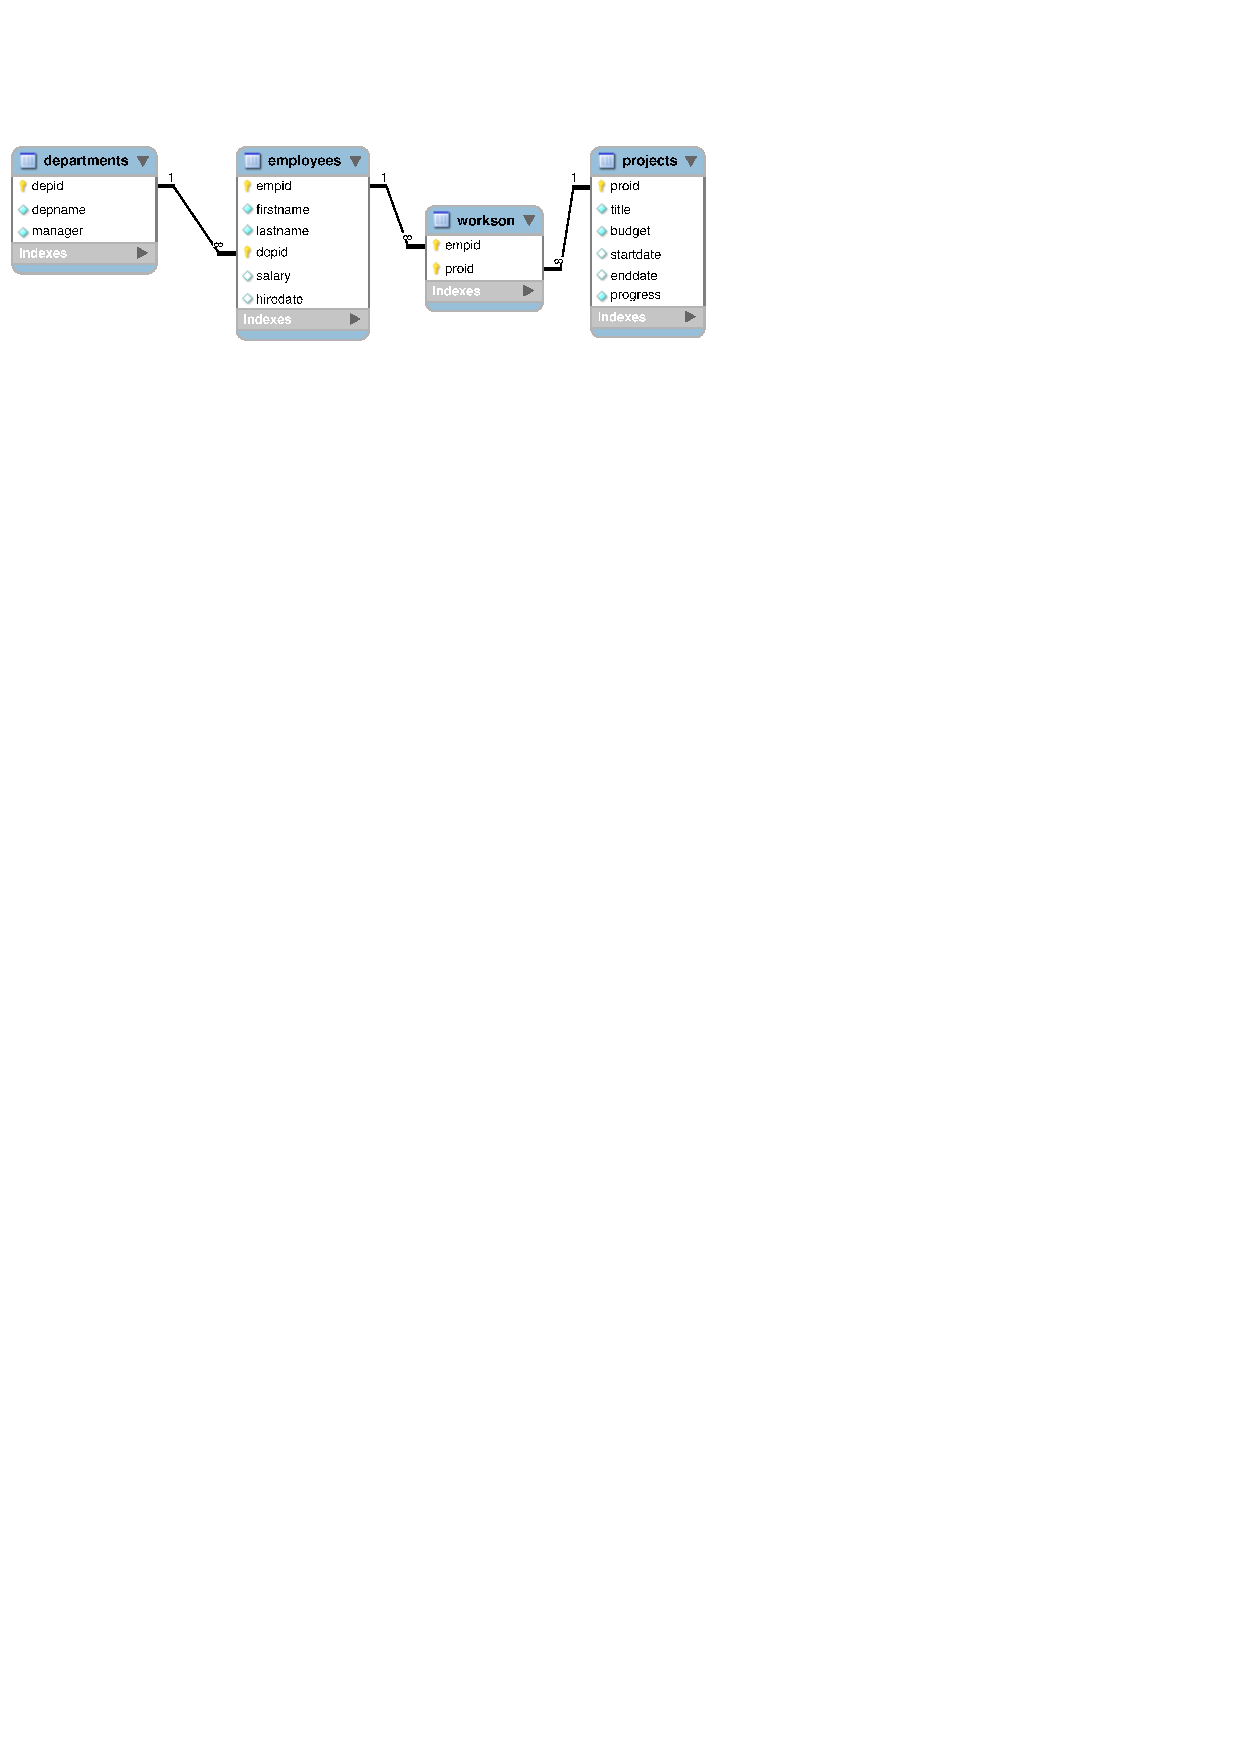
\includegraphics[scale=0.9]{../common/companyREL.pdf}
\vspace{0.5cm}
\begin{itemize} \itemsep 6pt
  \item {\ra departments}, τα τμήματα της εταιρείας.
  \item {\ra employees}, οι υπάλληλοι της εταιρείας.
  \item {\ra projects}, τα έργα που εκτελεί η εταιρεία.
  \item {\ra workson}, η απασχόληση των υπαλλήλων στα έργα.
\end{itemize}
\end{minipage}
\end{frame}
